\section{Friedmann Equation}
The Friedmann equation, describing the expansion of the universe, is one of the most important equations in cosmology. The equation can be derived completely from Newtonian theory, while General Relativity can be used to correct for outlying cases.

\subsection{Derivation}
Consider a particle of mass m at a distance r from a fixed point which may be assumed to be the centre of expansion, by virtue of the cosmological principle. The kinetic and potential energies of the particle will be given by:

\begin{center}
    $T = \frac{1}{2}m\dot{r}^2$ \\
\end{center}

\begin{center}
    $V = -\frac{GMm}{r} = -\frac{4\pi G \rho r^2 m}{3}$
\end{center}

Using Newton's laws, the total energy U \textbf{of the particle} given by the sum of potential and kinetic energies will be:

\begin{equation}
U = \frac{1}{2}m\dot{r}^2-\frac{4\pi}{3}G{\rho}r^2m
\end{equation}

The crucial step in the derivation is shifting the coordinates to a system called \textbf{comoving coordinates}, which can be expressed as $\vec{r}=a(t)\vec{x}$, where x is fixed for the particle under consideration, i.e $\dot{x}=0.$. Here a is known as the \textbf{scale factor of the Universe}, and gives information about how physical separation(r) changes with time.

\begin{figure}[H]
    \centering
    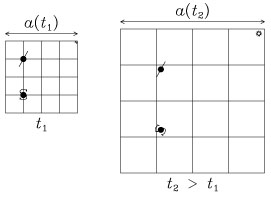
\includegraphics[width=0.5\textwidth]{figure1}
    \caption{Comoving coordinates}
    \label{fig:coord}
\end{figure}

\begin{center}
    $U = {\frac{1}{2}}{m{\dot{a}^2}{x^2}}-\frac{4\pi}{3}G{\rho}{a^2}{x^2}m$
\end{center}

Further simplification, after the above substitution, leads to the Friedmann equation:

\begin{equation} \label{eq:1}
(\frac{\dot{a}}{a})^2 = \frac{8{\pi}G}{3}\rho -\frac{kc^2}{a^2}
\end{equation}

The left hand side of the equation is independent of spatial coordinates, implying that $k = -\frac{2U}{m{c^2}{x^2}}$ must also be independent of x. Therefore $U \propto {x^2}$.The constant k, is related to the curvature of space and will be used extensively in further analysis. \\

NOTE: The expansion of the universe makes sense only at very large distance scales (such as at mega-parsec scale), as the universe is expected to appear uniform then. 

\subsection{Fluid and Acceleration equations}
Information about the mass density of the universe is necessary to obtain a solution of the Friedmann equation. This is given by a differential equation involving the pressure p, of material and is called the fluid equation. It can be obtained from the first law of thermodynamics: $dE+pdV = TdS $. I the comoving radius x is set to 1, then:

\begin{center}
    $E = mc^2 = \frac{4\pi}{3}a^3{\rho}c^2$ \\
\end{center}
    
\begin{center}    
    $\frac{dE}{dt} = 4{\pi}a^2{\rho}c^2\frac{da}{dt}+\frac{4\pi}{3}a^3c^2\frac{d\rho}{dt}$
\end{center}

Using $\frac{dV}{dt} = 4{\pi}a^2\frac{da}{dt}$ and assuming reversible adiabatic expansion (dS=0), the fluid equation comes out as:

\begin{equation} \label{eq:2}
    \dot{\rho}+3\frac{\dot{a}}{a}(\rho+\frac{p}{c^2})=0
\end{equation}

Although a pressure term appears in the above equation, it is important to note that in a homogeneous universe, no pressure gradients exist, implying that force does not aid in expansion of space. Pressure only contributes to work done.
\\
The acceleration equation can be obtained by differentiating equation \ref{eq:1} with respect to time and substituting $\dot{\rho}$ from \ref{eq:2}. This gives:

\begin{center}
    $\frac{\ddot{a}}{a}-(\frac{\dot{a}}{a})^2=-4{\pi}G(\rho+\frac{p}{c^2}+\frac{kc^2}{a^2}$
\end{center}

Substituting $\frac{\ddot{a}}{a}$ from equation \ref{eq:1} again, we obtain the \textbf{acceleration equation}:

\begin{equation}
    \frac{\ddot{a}}{a}=\frac{-4{\pi}G}{3}(\rho+\frac{3p}{c^2})
\end{equation}

Typically, the value of c is set to 1 in cosmology, making time and length, as well as mass and energy interchangeable. Hence the $c^2$ term in the Friedmann equation is often dropped, giving k the unit of $[time]^{-2}$.

\subsection{Interpretation of $k$}

The term $k$ which appears in the Friedmann equation is related to the curvature of space, in the purview of general relativity. Corresponding the different values of $k$, different goementries are possible for the universe; namely flat (corresponding to $k$=0), spherical (corresponding to $k>0$) and hyperbolic (corresponding to $k<0$).

\begin{itemize}
    \item Flat geometry: As is clear from the name, this would correspond to a two dimensional plane universe, where Euclidean geometry principles hold (the shortest distance between two point is a straight line and parallel lines are e fixed distance apart). This is usually called \textbf{flat universe}.
    \item Spherical geometry: This corresponds to a closed structure, with no boundary and fixed area, where Euclidean axioms do not hold. In fact it is one of the simplest non-Euclidean geometries known. The symmetry of the sphere preserves isotropy as well. This case is referred to as \textbf{closed universe}.
    \item Hyperbolic geometry: This represents a saddle type structure which, again, does not satisfy Euclidean norms and 'parallel lines' diverge from each other. This is referred to as \textbf{open universe}.
\end{itemize}

The open and flat would mean that the universe is infinite at any finite time. It could still continue expanding in the sense that distance between objects in it continue to increase. There is no way to confirm whether this is the case as we can only see a small part of the universe, restricted by the speed of light, known as the \textbf{observable universe}.

\begin{figure}[H]
    \centering
    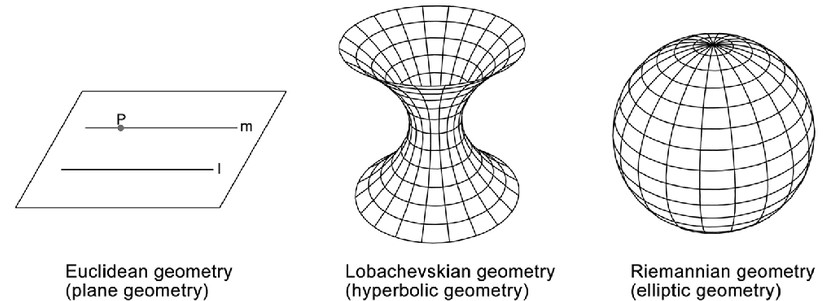
\includegraphics[width=\textwidth]{figure 4.jpg}
    \caption{These are the three postulated geometries of the universe corresponding to different values of $k$, as described above}
    \label{fig:matrad}
\end{figure}
